\begin{prob}[(17 pts)]

\begin{subprobset}

\begin{subprob}(5 pts) Complete the implementation of the function \texttt{most\_sunshine}, which takes in \texttt{country}, the name of a country, and \texttt{month}, the name of a month (e.g. \texttt{"Apr"}), and returns the name of the city (as a string) in \texttt{country} with the most sunshine hours in \texttt{month}, among the cities in \texttt{sun}. Assume there are no ties.

\begin{verbatim}
def most_sunshine(country, month):
    country_only = __(a)__
    return country_only.__(b)__
\end{verbatim}

What goes in blank (a)?

\begin{responsebox}{0.5in}
    
\end{responsebox}

What goes in blank (b)?

\begin{responsebox}{1in}
    
\end{responsebox}
    
\end{subprob}

\begin{subprob}(4 pts) In this part only, assume that all \texttt{"City"} names in \texttt{sun} are unique.

Consider the DataFrame \texttt{cities} defined below.

\begin{verbatim}
cities = sun.groupby("City").mean().reset_index()
\end{verbatim}

Fill in the blanks so that the DataFrame that results from the sequence of steps described below is identical to \texttt{cities}.

\begin{center}
``Sort \texttt{sun} by \_\_(c)\_\_ in \_\_(d)\_\_ order \_\_(e)\_\_."
\end{center}

What goes in blank (c)?

\bubble{\texttt{"Country"}}
\bubble{\texttt{"City"}}
\bubble{\texttt{"Jan"}}
\bubble{\texttt{"Year"}}

\vspace{.1in}

What goes in blank (d)?

\bubble{ascending}
\bubble{descending}

\vspace{.1in}

What goes in blank (e)?

\bubble{and drop the \texttt{"Country"} column}

\bubble{and drop the \texttt{"Country"} and \texttt{"City"} columns}

\bubble{and reset the index}

\bubble{, drop the \texttt{"Country"} column, and reset the index}

\bubble{, drop the \texttt{"Country"} and \texttt{"City"} columns, and reset the index}

\bubble{Nothing, leave blank (e) empty}

\end{subprob}

\newpage

\begin{subprob}(2 pts) True or False: In the code below, \texttt{Z} is guaranteed to evaluate to \texttt{True}.
\begin{verbatim}
x = sun.groupby(["Country", "Year"]).mean().shape[0]
y = sun.groupby("Country").mean().shape[0]
z = (x >= y)
\end{verbatim}

\bubble{True}
\bubble{False}

\end{subprob}

\end{subprobset}

In the next few parts, consider the following answer choices.

\begin{enumerate}[label=\Alph*.]
    \item The name of the country with the most cities.
    
    \item The name of the country with the fewest cities.
    
    \item The number of cities in the country with the most cities.
    
    \item The number of cities in the country with the fewest cities.
    
    \item The last city, alphabetically, in the first country, alphabetically.
    
    \item The first city, alphabetically, in the first country, alphabetically.
    
    \item Nothing, because it errors.
\end{enumerate}

\begin{subprobset}

\begin{subprob}(1.5 pts) What does the following expression evaluate to?

\begin{verbatim}
sun.groupby("Country").max().get("City").iloc[0]
\end{verbatim}

\bubble{A}
\bubble{B}
\bubble{C}
\bubble{D}
\bubble{E}
\bubble{F}
\bubble{G}

\end{subprob}

\begin{subprob}(1.5 pts) What does the following expression evaluate to?

\begin{verbatim}
sun.groupby("Country").sum().get("City").iloc[0]
\end{verbatim}

\bubble{A}
\bubble{B}
\bubble{C}
\bubble{D}
\bubble{E}
\bubble{F}
\bubble{G}

\end{subprob}

\begin{subprob}(1.5 pts) What does the following expression evaluate to?
\begin{verbatim}
sun.groupby("Country").count().sort_values("Jan").index[-1]
\end{verbatim}

\bubble{A}
\bubble{B}
\bubble{C}
\bubble{D}
\bubble{E}
\bubble{F}
\bubble{G}

\end{subprob}

\begin{subprob}(1.5 pts) What does the following expression evaluate to?
\begin{verbatim}
sun.groupby("Country").count().sort_values("City").get("City").iloc[-1]
\end{verbatim}

\bubble{A}
\bubble{B}
\bubble{C}
\bubble{D}
\bubble{E}
\bubble{F}
\bubble{G}

\end{subprob}
   
\end{subprobset}

\end{prob}

\newpage

\begin{prob}[(7 pts)]

Vanessa is a big Formula 1 racing fan, and wants to plan a trip to Monaco, where the Monaco Grand Prix is held. Monaco is an example of a ``city-state" --- that is, a city that is its own country. Singapore is another example of a city-state.

We'll say that a row of \texttt{sun} corresponds to a city-state if its \texttt{"Country"} and \texttt{"City"} values are equal.

\begin{subprobset}

\begin{subprob}(4 pts) Fill in the blanks so that the expression below is equal to the total number of sunshine hours in October of all city-states in \texttt{sun}.

\begin{verbatim}
sun[__(a)__].__(b)__
\end{verbatim}

What goes in blank (a)?

\begin{responsebox}{0.5in}
    
\end{responsebox}

What goes in blank (b)?

\begin{responsebox}{0.5in}
    
\end{responsebox}

\end{subprob}

\begin{subprob}(3 pts) Fill in the blanks below so that the expression below is also equal to the total number of sunshine hours in October of all city-states in \texttt{sun}.

\textit{Note: What goes in blank (b) is the same as what goes in blank (b) above.}

\begin{verbatim}
sun.get(["Country"]).merge(__(c)__).__(b)__
\end{verbatim}

What goes in blank (c)?

\begin{responsebox}{0.5in}
    
\end{responsebox}

\end{subprob}
    
\end{subprobset}

\end{prob}

\newpage

\begin{prob}[(13 pts)]

This summer, Zoe wants to explore parts of the United States that she hasn't been to yet. In her process of figuring out where to go, she creates a histogram depicting the distribution of the number of sunshine hours in July across all cities in the United States in \texttt{sun}.

\begin{center}
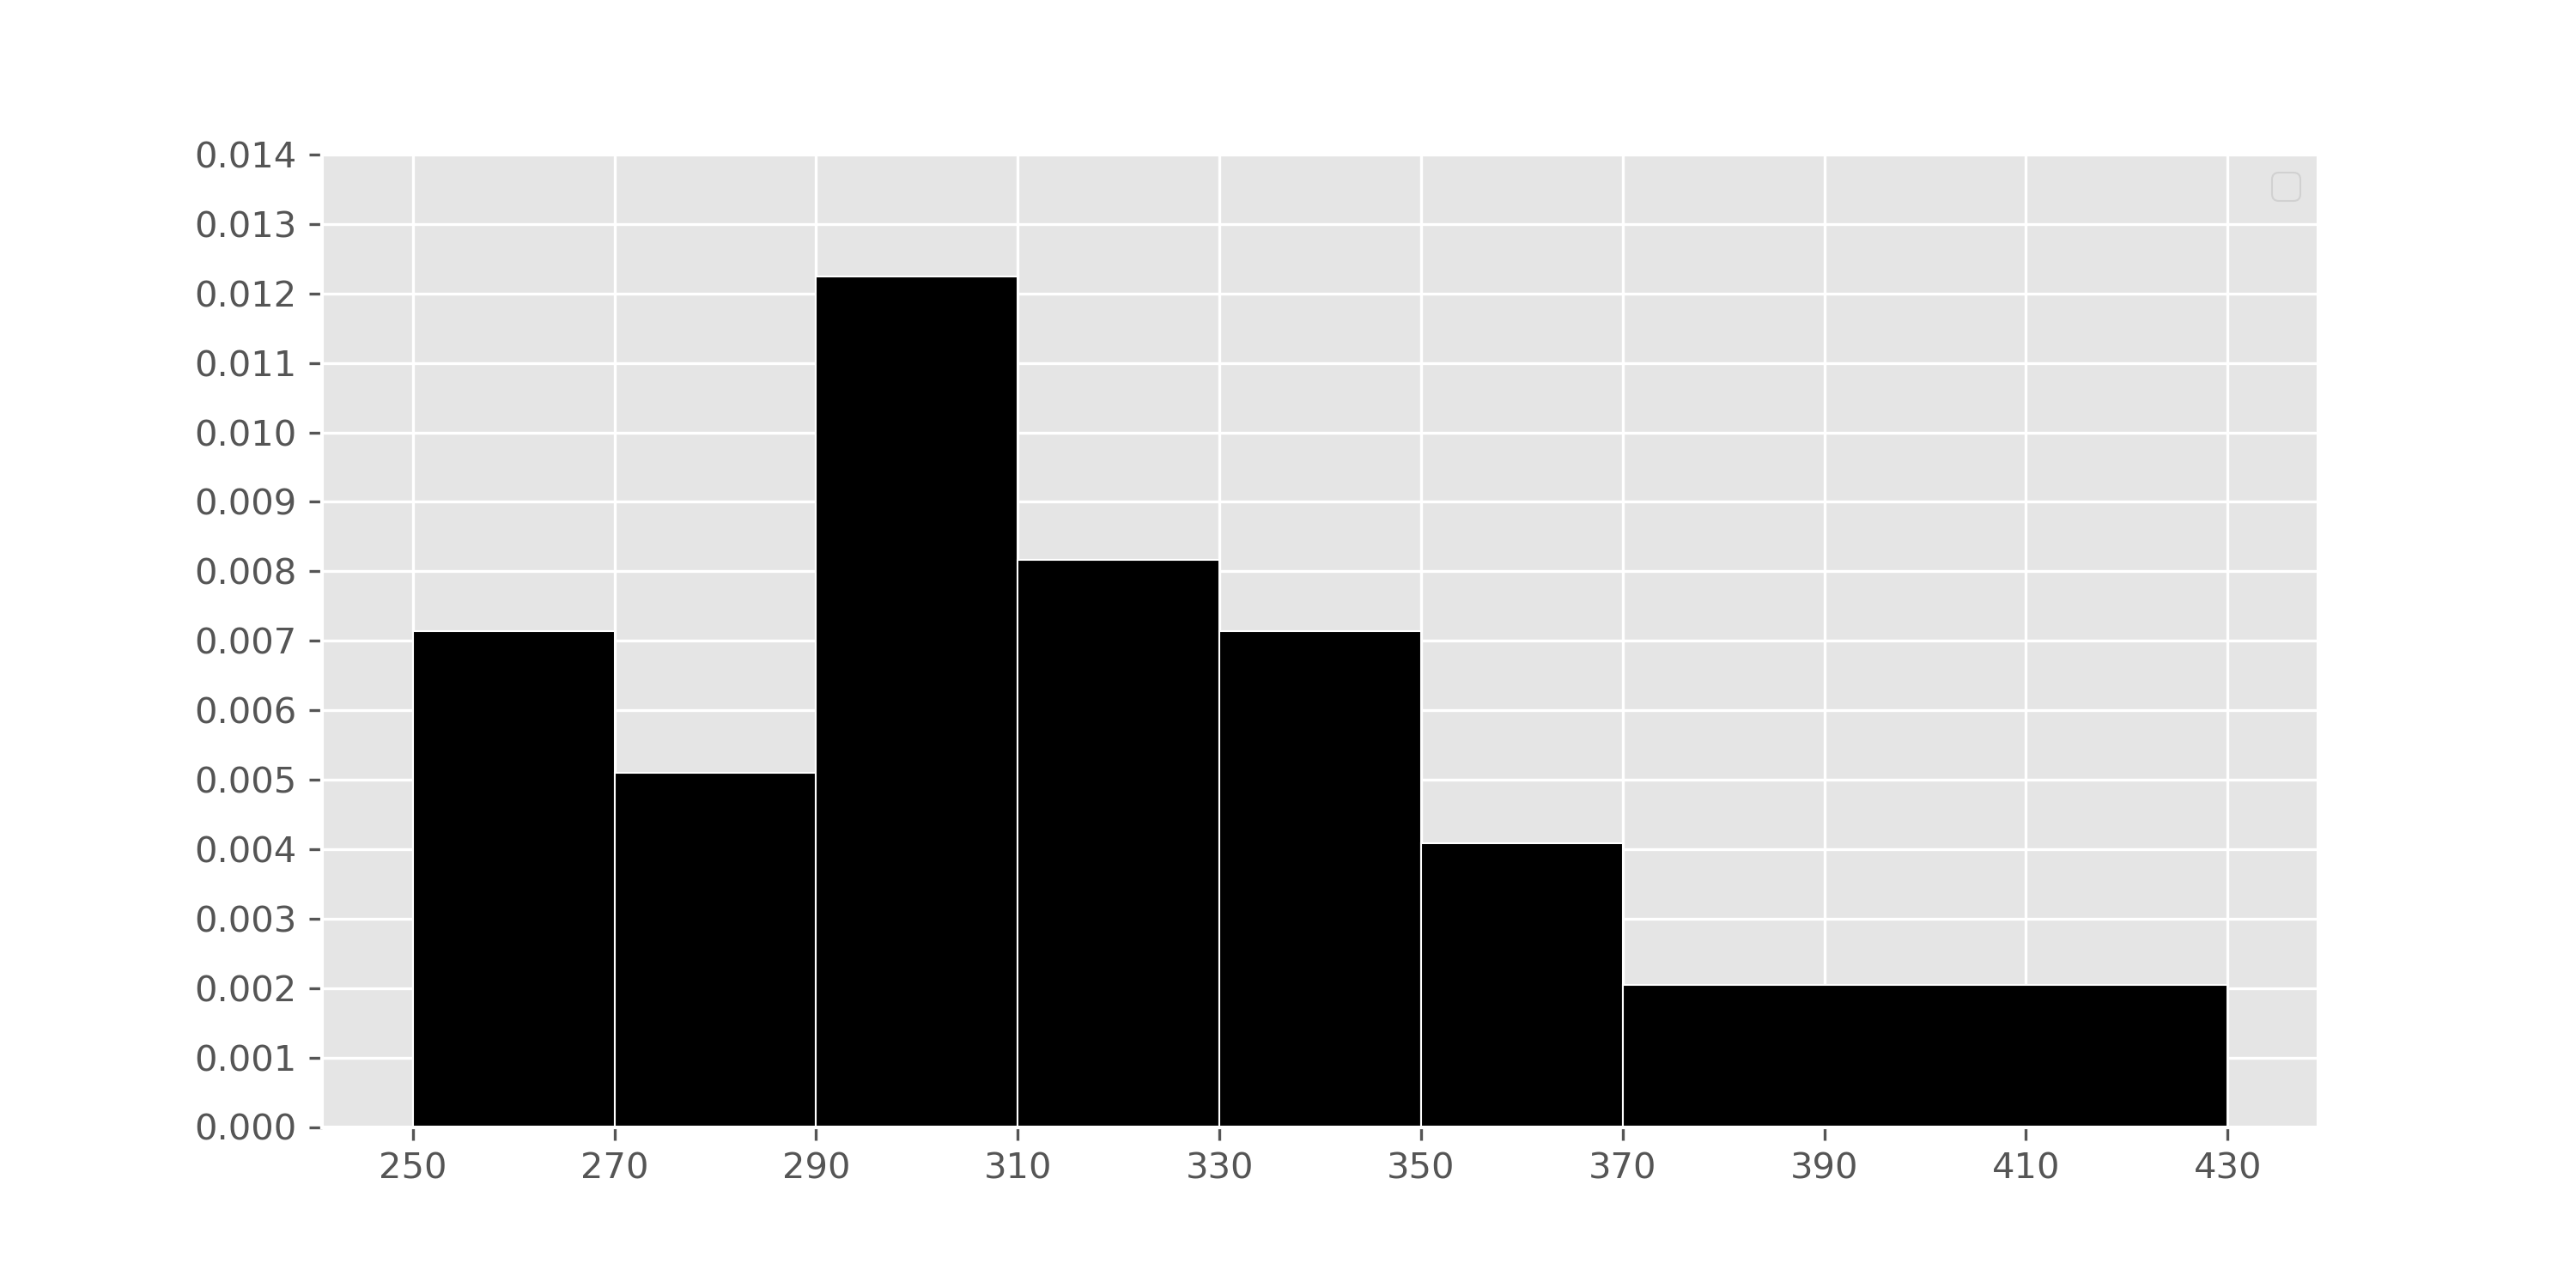
\includegraphics[width=\textwidth]{final_images/america-hist.png}
\end{center}

Suppose \texttt{usa} is a DataFrame with all of the columns in \texttt{sun} but with only the rows where \texttt{"Country"} is \texttt{"United States"}.


\begin{subprobset}

\begin{subprob}(3 pts) What is the value of \texttt{mystery} below?

\begin{verbatim}
cond = (usa.get("Jul") >= 370) & (usa.get("Jul") < 430)
mystery = 100 * np.count_nonzero(cond) / usa.shape[0]
\end{verbatim}

\bubble{\texttt{2}}
\bubble{\texttt{8}}
\bubble{\texttt{12}}
\bubble{\texttt{16}}
\bubble{\texttt{18}}
\bubble{\texttt{20}}
    
\end{subprob}

% \begin{subprob}

% The histogram drawn above has 7 bars. Suppose we created a new histogram with the same numbers but with only two bars: $[250, 370)$ and $[370, 430)$. What would the height of the new $[250, 370)$ bar be? Assume that the height of the $[370, 430)$ bar in the histogram above is exactly 0.002.
    
% \end{subprob}

\begin{subprob}(4 pts) There are 3 more cities with between 370 and 430 sunshine hours in July than there are cities with between 270 and 290 sunshine hours in July.

How many cities in the United States are in \texttt{sun}? Give your answer as a positive integer, rounded to the nearest multiple of 10 (that is, your answer should end in a 0).

\inlineresponsebox[2in]{}{}

\end{subprob}

\end{subprobset}

\newpage

Now, suppose we convert the number of sunshine hours in July for all cities in the United States (i.e., ``US cities") in \texttt{sun} from their original units (hours) to standard units.

\begin{subprobset}

\begin{subprob}(1.5 pts) Let $m$ be the mean number of sunshine hours in July for all US cities in \texttt{sun}, in standard units. Select the true statement below.

\begin{tabular}{lll}
\bubble{$m = -1$} & \bubble{$-1 < m < 0$} &  \bubble{$m = 0$} \\ 
\bubble{$0 < m < 1$} & \bubble{$m = 1$} & \bubble{$m > 1$}
\end{tabular}

\end{subprob}

\begin{subprob}(1.5 pts) Let $s$ be the standard deviation of the number of sunshine hours in July for all US cities \texttt{sun}, in standard units. Select the true statement below.

\begin{tabular}{lll}
\bubble{$s = -1$} & \bubble{$-1 < s < 0$} &  \bubble{$s = 0$} \\ 
\bubble{$0 < s < 1$} & \bubble{$s = 1$} & \bubble{$s > 1$}
\end{tabular}

\end{subprob}

\begin{subprob}(1.5 pts) Let $d$ be the median of the number of sunshine hours in July for all US cities in \texttt{sun}, in standard units. Select the true statement below.

\begin{tabular}{lll}
\bubble{$d = -1$} & \bubble{$-1 < d < 0$} &  \bubble{$d = 0$} \\ 
\bubble{$0 < d < 1$} & \bubble{$d = 1$} & \bubble{$d > 1$}
\end{tabular}

\end{subprob}

\begin{subprob}(1.5 pts) True or False: The distribution of the number of sunshine hours in July for all US cities in \texttt{sun}, in standard units, is roughly normal.

\bubble{True}
\bubble{False}
\bubble{Impossible to tell}

\end{subprob}
    
\end{subprobset}


\end{prob}

\newpage

\begin{prob}[(8 pts)]

For each city in \texttt{sun}, we have 12 numbers, corresponding to the number of sunshine hours it sees in January, February, March, and so on, through December. (There is also technically a 13th number, the value in the \texttt{"Year"} column, but we will ignore it for the purposes of this question.)

We say that a city's number of sunshine hours \textbf{peaks gradually} if both of the following conditions are true:
\begin{itemize}
    \item Each month from February to June has a number of sunshine hours greater than or equal to the month before it.
    \item Each month from August to December has a number of sunshine hours less than or equal to the month before it.
\end{itemize}

For example, the number of sunshine hours per month in Doris' hometown of Guangzhou, China peaks gradually:

$$62, 65, 71, 104, 118, 202, 181, 173, 172, 170, 166, 140$$

However, the number of sunshine hours per month in Charlie's hometown of Redwood City, California does not peak gradually, since $325 > 311$ and $247 < 271$:

$$185, 207, 269, 309, 325, 311, 313, 287, 247, 271, 173, 160$$

Complete the implementation of the function \texttt{peaks\_gradually}, which takes in an array \texttt{hours} of length 12 corresponding to the number of sunshine hours per month in a city, and returns \texttt{True} if the city's number of sunshine hours peaks gradually and \texttt{False} otherwise.

\begin{verbatim}
def peaks_gradually(hours):
    for i in np.arange(5):
        cur_left = hours[5 - i]
        next_left = hours[__(a)__]
        cur_right = hours[__(b)__]
        next_right = hours[6 + i + 1]

        if __(c)__:
            __(d)__
        
    __(e)__
\end{verbatim}

\newpage

\begin{subprobset}

\begin{subprob}(2 pts) What goes in blank (a)?

\begin{responsebox}{0.5in}
    
\end{responsebox}
    
\end{subprob}

\begin{subprob}(2 pts) What goes in blank (b)?

\begin{responsebox}{0.5in}
    
\end{responsebox}
    
\end{subprob}

\begin{subprob}(2 pts) What goes in blank (c)?

\bubble{\texttt{next\_left < cur\_left or next\_right < cur\_right}}

\bubble{\texttt{next\_left < cur\_left and next\_right < cur\_right}}

\bubble{\texttt{next\_left > cur\_left or next\_right > cur\_right}}

\bubble{\texttt{next\_left > cur\_left and next\_right > cur\_right}}
    
\end{subprob}

\begin{subprob}(1 pt) What goes in blank (d)?

\bubble{\texttt{return True}}
\bubble{\texttt{return False}}

\end{subprob}

\begin{subprob}(1 pt) What goes in blank (e)?

\bubble{\texttt{return True}}
\bubble{\texttt{return False}}

\end{subprob}

    
\end{subprobset}

\end{prob}

\newpage

\begin{prob}[(11 pts)]

In some cities, the number of sunshine hours per month is relatively consistent throughout the year. São Paulo, Brazil is one such city; in all months of the year, the number of sunshine hours per month is somewhere between 139 and 173. New York City's, on the other hand, ranges from 139 to 268.

Gina and Abel, both San Diego natives, are interested in assessing how ``consistent" the number of sunshine hours per month in San Diego appear to be. Specifically, they'd like to test the following hypotheses:

\begin{itemize}
    \item \textbf{Null Hypothesis}: The number of sunshine hours per month in San Diego is drawn from the uniform distribution, $\left[\frac{1}{12}, \frac{1}{12}, ..., \frac{1}{12}\right]$. (In other words, the number of sunshine hours per month in San Diego is equal in all 12 months of the year.) 
    \item \textbf{Alternative Hypothesis}: The number of sunshine hours per month in San Diego is not drawn from the uniform distribution.
\end{itemize}

As their test statistic, Gina and Abel choose the total variation distance. To simulate samples under the null, they will sample from a categorical distribution with 12 categories --- January, February, and so on, through December --- each of which have an equal probability of being chosen.

% \begin{itemize}
%     \item Model distribution: 
%     \item Example sample distribution: $\left[\frac{3}{14}, \frac{1}{9}, ..., \frac{1}{12}\right]$
% \end{itemize}

\begin{subprobset}

% \begin{subprob}
% This week, there have been massive wildfires in Eastern Canada, leading to smokier skies and fewer sunshine hours in much of the East Coast. Fortunately, these fires have not reached the part of Canada where Suraj is from. Unfortunately, we've seen such wildfires and cloudy conditions in California before.

% Suppose that the wildfire situation dramatically escalates across the country and that in 2024, San Diego only sees 225 total sunshine hours the whole year, all of them coming in the month of September. (That is, there is 0 sunshine in all other months combined.) What is the TVD between San Diego's 2024 distribution of sunshine hours per month and the uniform distribution?

% \bubble{$\frac{5}{12}$} \bubble{$\frac{5}{11}$} \bubble{$\frac{1}{2}$} \bubble{$\frac{6}{11}$} \bubble{$\frac{11}{12}$} \bubble{$1$} \bubble{$\frac{11}{6}$}

% \end{subprob}

\begin{subprob}(2 pts) In order to run their hypothesis test, Gina and Abel need a way to calculate their test statistic. Below is an incomplete implementation of a function that computes the TVD between two arrays of length 12, each of which represent a categorical distribution.

\begin{verbatim}
def calculate_tvd(dist1, dist2):
    return np.mean(np.abs(dist1 - dist2)) * ____
\end{verbatim}

Fill in the blank so that \texttt{calculate\_tvd} works as intended.

\bubble{\texttt{1 / 6}}
\bubble{\texttt{1 / 3}}
\bubble{\texttt{1 / 2}}
\bubble{\texttt{2}}
\bubble{\texttt{3}}
\bubble{\texttt{6}}

\end{subprob}

\end{subprobset}

\textbf{Moving forward, assume that \texttt{calculate\_tvd} works correctly.}

\newpage

Now, complete the implementation of the function \texttt{uniform\_test}, which takes in an array \texttt{observed\_counts} of length 12 containing the number of sunshine hours each month in a city and returns the p-value for the hypothesis test stated at the start of the question.

\begin{verbatim}
def uniform_test(observed_counts):
    # The values in observed_counts are counts, not proportions!
    total_count = observed_counts.sum()
    uniform_dist = __(b)__
    tvds = np.array([])
    for i in np.arange(10000):
        simulated = __(c)__
        tvd = calculate_tvd(simulated, __(d)__)
        tvds = np.append(tvds, tvd)
    return np.mean(tvds __(e)__ calculate_tvd(uniform_dist, __(f)__))
\end{verbatim}

\begin{subprobset}

\begin{subprob}(2 pts) What goes in blank (b)? \textit{(Hint: The function \texttt{np.ones(k)} returns an array of length \texttt{k} in which all elements are \texttt{1}.)}

\begin{responsebox}{0.5in}
    
\end{responsebox}
   
\end{subprob}

\begin{subprob}(2 pts) What goes in blank (c)?

\bubble{\texttt{np.random.multinomial(12, uniform\_dist)}}

\bubble{\texttt{np.random.multinomial(12, uniform\_dist) / 12}}

\bubble{\texttt{np.random.multinomial(12, uniform\_dist) / total\_count}}

\bubble{\texttt{np.random.multinomial(total\_count, uniform\_dist)}}

\bubble{\texttt{np.random.multinomial(total\_count, uniform\_dist) / 12}}

\bubble{\texttt{np.random.multinomial(total\_count, uniform\_dist) / total\_count}}
   
\end{subprob}

\begin{subprob}(2 pts) What goes in blank (d)?

\begin{responsebox}{0.5in}
    
\end{responsebox}

\end{subprob}

\begin{subprob}(1 pt) What goes in blank (e)?

\bubble{\texttt{>}}
\bubble{\texttt{>=}}
\bubble{\texttt{<}}
\bubble{\texttt{<=}}
\bubble{\texttt{==}}
\bubble{\texttt{!=}}

\end{subprob}

\begin{subprob}(2 pts) What goes in blank (f)?

\begin{responsebox}{0.5in}
    
\end{responsebox}

\end{subprob}
    
\end{subprobset}

% something about choice vs. np.random.multinomial

\end{prob}

% \newpage

% \begin{prob}
% Due to its northern latitude, Iceland is known for having extremely long days in the summer --- for a few straight months, the sun never sets!

% Abel is planning on road tripping through Iceland this summer and wants to estimate the proportion of cities in Iceland that will see over 400 sunshine hours this July. To do so, he plans on visiting many Icelandic cities before July starts and installing solar sensors in each city, which will allow him to track the number of sunshine hours in July in each city.

% Ultimately, he'd like to produce a 99.73\% confidence interval for the proportion of cities that see over 400 sunshine hours in July. After doing some research, he learns that this proportion is guaranteed to be at least $\frac{5}{8}$. He wants to guarantee that the width of his confidence interval is less than or equal to $\frac{1}{16}$.

% Let $n$ be the smallest number of cities Abel must visit to guarantee that  his 99.73\% confidence interval has his desired width. $n$ is a multiple of 15, meaning that it is of the form $15 k$, where $k$ is some positive integer. What is the value of $k$?

% \textit{Hints: \begin{itemize}
%     \item Under the standard normal distribution, 99.73\% of values fall within 3 standard deviations of the mean.
%     \item In a collection of 0s and 1s, the standard deviation is $$\sqrt{\text{(Proportion of 0s)} \cdot \text{(Proportion of 1s)}}$$ In lecture, we learned that the maximum possible standard deviation of a collection of 0s and 1s, given no other information, is $\frac{1}{2}$. Given the information in this question, you can find the maximum possible standard deviation of Abel's sample, and it is less than $\frac{1}{2}$. \textbf{The first step to answering the overall question is finding the maximum possible standard deviation of Abel's sample.}
%     \item For example, if you think the smallest number of cities Abel must visit is 45, you would answer 3, because $15 \cdot 3 = 45$. We've set the question up in this way so that you don't actually need to perform the final arithmetic calculation yourself without a calculator.
% \end{itemize}}

% $k = $ \inlineresponsebox[2in]{}{}

% % Show your work in the box below. We \textit{may} award partial credit for incorrect answers with correct steps shown.

% % \begin{responsebox}{2in}
    
% % \end{responsebox}

% \end{prob}

\newpage

\begin{prob}[(17 pts)]

Oren's favorite bakery in San Diego is Wayfarer. After visiting frequently, he decides to learn how to make croissants and baguettes himself, and to do so, he books a trip to France.

Oren is interested in estimating the mean number of sunshine hours in July across all 10,000+ cities in France. Using the 16 French cities in \texttt{sun}, Oren constructs a 95\% Central Limit Theorem (CLT)-based confidence interval for the mean sunshine hours of all cities in France. The interval is of the form $[L, R]$, where $L$ and $R$ are positive numbers.

\begin{subprobset}

\begin{subprob}(3 pts) Which of the following expressions is equal to the standard deviation of the number of sunshine hours of the 16 French cities in \texttt{sun}?

\bubble{$R - L$}
\bubble{$\frac{R - L}{2}$}
\bubble{$\frac{R - L}{4}$}
\bubble{$R + L$}
\bubble{$\frac{R + L}{2}$}
\bubble{$\frac{R + L}{4}$}

\end{subprob}

\begin{subprob}(1.5 pts) True or False: There is a 95\% chance that the interval $[L, R]$ contains the mean number of sunshine hours in July of all 16 French cities in \texttt{sun}.

\bubble{True}
\bubble{False}

\end{subprob}

\begin{subprob}(1.5 pts) True or False: If we collected 1,000 new samples of 16 French cities and computed the mean of each sample, then about 95\% of the new sample means would be contained in $[L, R]$.

\bubble{True}
\bubble{False}

\end{subprob}

\begin{subprob}(1.5 pts) True or False: If we collected 1,000 new samples of 16 French cities and created a 95\% confidence interval using each one, then chose one of the 1,000 new intervals at random, the chance that the randomly chosen interval contains the mean sunshine hours in July across all cities in France is approximately 95\%.

\bubble{True}
\bubble{False}

\end{subprob}

\begin{subprob}(1.5 pts) True or False: The interval $[L, R]$ is centered at the mean number of sunshine hours in July across all cities in France.

\bubble{True}
\bubble{False}

\end{subprob}

\end{subprobset}

\newpage

In addition to creating a 95\% CLT-based confidence interval for the mean sunshine hours of all cities in France, Oren would like to create a 76\% bootstrap-based confidence interval for the mean sunshine hours of all cities in France.

Oren resamples from the 16 French sunshine hours in \texttt{sun} 10,000 times and creates an array named \texttt{french\_sunshine} containing 10,000 resampled means. He wants to find the left and right endpoints of his 76\% confidence interval:

\begin{verbatim}
boot_left = np.percentile(french_sunshine, __(a)__)
boot_right = np.percentile(french_sunshine, __(b)__)
\end{verbatim}

\begin{subprobset}

\begin{subprob}(4 pts) Fill in the blanks so that \texttt{boot\_left} and \texttt{boot\_right} evaluate to the left and right endpoints of a 76\% confidence interval for the mean sunshine hours in July across all cities in France.

\begin{minipage}[t]{0.4\textwidth}
What goes in blank (a)?

\inlineresponsebox[2in]{}{}
\end{minipage}
\hfill
\begin{minipage}[t]{0.4\textwidth}
What goes in blank (b)?

\inlineresponsebox[2in]{}{}
\end{minipage}

\end{subprob}

\end{subprobset}

Suppose we are interested in testing the following pair of hypotheses.

\begin{itemize}
    \item \textbf{Null Hypothesis}: The mean number of sunshine hours of all cities in France in July is equal to 225.
    \item \textbf{Alternative Hypothesis}: The mean number of sunshine hours of all cities in France in July is not equal to 225.
\end{itemize}

% We say a confidence interval $X$ is \textit{contained} within another confidence interval $Y$ if $X$'s left endpoint is greater than $Y$'s left endpoint and $X$'s right endpoint is less than $Y$'s right endpoint.

% In the following example, Intervals 2 and 3 are both contained within Interval 1.

% \begin{center}
% 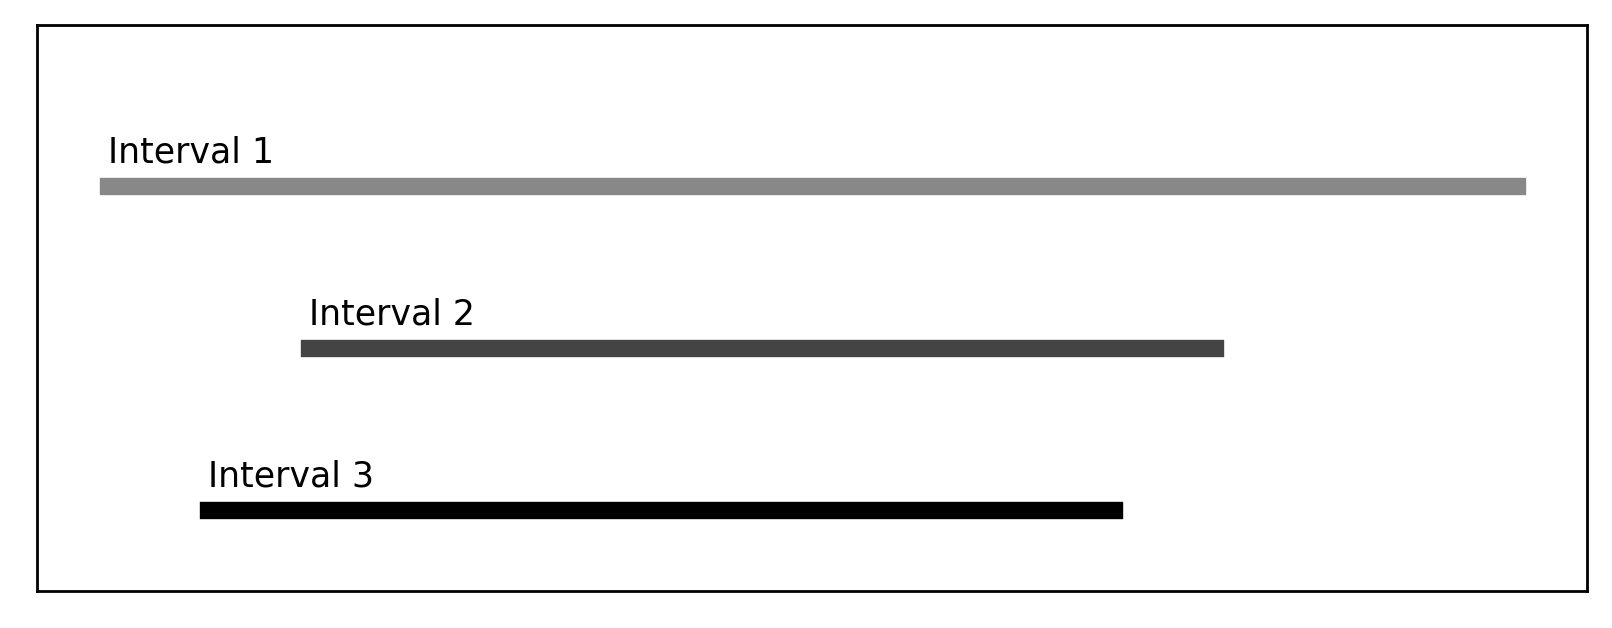
\includegraphics[width=0.7\textwidth]{final_images/intervals.png}
% \end{center}

\begin{subprobset}

\begin{subprob}(1.5 pts) Suppose that when Oren uses \texttt{[boot\_left, boot\_right]}, his 76\% bootstrap-based confidence interval, he fails to reject the null hypothesis above. If that's the case, then when using $[L, R]$, his 95\% CLT-based confidence interval, what is the conclusion of his hypothesis test?

\bubble{Reject the null}
\bubble{Fail to reject the null}
\bubble{Impossible to tell}

\end{subprob}

\begin{subprob}(1.5 pts) Suppose that Oren also creates a 76\% CLT-based confidence interval for the mean sunshine hours of all cities in France in July using the same 16 French cities in \texttt{sun} he started with. When using his 76\% CLT-based confidence interval, he fails to reject the null hypothesis above. If that's the case, then when using $[L, R]$, what is the conclusion of his hypothesis test?

\bubble{Reject the null}
\bubble{Fail to reject the null}
\bubble{Impossible to tell}

\end{subprob}

\begin{subprob}(1 pt) True or False: The significance levels of both hypothesis tests described in part (h) are equal.

\bubble{True}
\bubble{False}

\end{subprob}

\end{subprobset}

\end{prob}

\newpage

\begin{prob}[(8 pts)]

Gabriel is originally from Texas and is trying to convince his friends that Texas has better weather than California. Sophia, who is originally from San Diego, is determined to prove Gabriel wrong.

Coincidentally, both are born in February, so they decide to look at the mean number of sunshine hours of all cities in California and Texas in February. They find that the mean number of sunshine hours for California cities in February is 265, while the mean number of sunshine hours for Texas cities in February is 250. They decide to test the following hypotheses:

\begin{itemize}
    \item \textbf{Null Hypothesis}: The distribution of sunshine hours in February for cities in California and Texas are drawn from the same population distribution.
    \item \textbf{Alternative Hypothesis}: The distribution of sunshine hours in February for cities in California and Texas are not drawn from the same population distribution; rather, California cities see more sunshine hours in February on average than Texas cities.
\end{itemize}

The test statistic they decide to use is:

$$\text{mean sunshine hours in California cities – mean sunshine hours in Texas cities}$$

\vspace{.1in}

To simulate data under the null, Sophia proposes the following plan:
\begin{enumerate}
    \item Count the number of Texas cities, and call that number \texttt{t}. Count the total number of cities in both California and Texas, and call that number \texttt{n}.
    \item Find the total number of sunshine hours across all California and Texas cities in February, and call that number \texttt{total}.
    \item Take a random sample of \texttt{t} sunshine hours from the entire sequence of California and Texas sunshine hours in February in the dataset. Call this random sample \texttt{t\_samp}.
    \item Find the difference between the mean of the values that are not in \texttt{t\_samp} (the California sample) and the mean of the values that are in \texttt{t\_samp} (the Texas sample).
\end{enumerate}

\begin{subprobset}

\begin{subprob}(1.5 pts) What type of test is this?

\bubble{Hypothesis test}
\bubble{Permutation test}
    
\end{subprob}
    
\end{subprobset}


\newpage

Complete the implementation of the function \texttt{one\_stat}, which takes in a DataFrame \texttt{df} that has two columns --- \texttt{"State"}, which is either \texttt{"California"} or \texttt{"Texas"}, and \texttt{"Feb"}, which contains the number of sunshine hours in February for each city --- and returns a single simulated test statistic using Sophia's plan.

\begin{verbatim}
def one_stat(df):
    # You don't need to fill in the ...,
    # assume we've correctly filled them in so that
    # texas_only has only the "Texas" rows from df.
    texas_only = ...
    t = texas_only.shape[0]
    n = df.shape[0]
    
    total = df.get("Feb").sum()
    
    t_samp = np.random.choice(df.get("Feb"), t, __(b)__)
    
    c_mean = __(c)__
    t_mean = t_samp.sum() / t
    return c_mean - t_mean
\end{verbatim}

\begin{subprobset}

\begin{subprob}(1.5 pts) What goes in blank (b)?

\bubble{\texttt{replace=True}}
\bubble{\texttt{replace=False}}
    
\end{subprob}

\begin{subprob}(3 pts) What goes in blank (c)? \textit{(Hint: Our solution uses 4 of the variables that are defined before \texttt{c\_mean}.)}

\begin{responsebox}{0.75in}
    
\end{responsebox}
    
\end{subprob}

\end{subprobset}

Fill in the blanks below to accurately complete the provided statement.

\begin{center}
``If Sophia and Gabriel want to test the null hypothesis that the mean number of sunshine hours in February in the two states is equal using a different tool, they could use bootstrapping to create a confidence interval for the true value of the test statistic they used in the above test and check whether \_\_(d)\_\_ is in the interval."

\end{center}

\begin{subprobset}

\begin{subprob}(2 pts) What goes in blank (d)? Your answer should be a specific number.

\inlineresponsebox[2in]{}{}
    
\end{subprob}

\end{subprobset}
    
\end{prob}

\newpage

\begin{prob}[(10 pts)]

Australia is in the southern hemisphere, meaning that its summer season is from December through February, when we have our winter. As a result, January is typically one of the sunniest months in Australia!

Arjun is a big fan of the movie Kangaroo Jack and plans on visiting Australia this January. In doing his research on where to go, he found the number of sunshine hours in January for the 15 Australian cities in \texttt{sun} and sorted them in \textbf{descending} order.

$$356, 337, 325, 306, 294, 285, 285, 266, 263, 257, 255, 254, 220, 210, 176$$

Throughout this question, use the mathematical definition of percentiles presented in class.

\begin{subprobset}

\begin{subprob}(2 pts) What is the 80th percentile of the collection of numbers above?

\bubble{254}
\bubble{255}
\bubble{294}
\bubble{306}
\bubble{325}
\bubble{337}

\end{subprob}

\begin{subprob}(3 pts) What is the \textbf{largest} positive integer $p$ such that 257 is the $p$th percentile of the collection of numbers above?

\inlineresponsebox[2in]{}{}

\end{subprob}

\begin{subprob}(3 pts) What is the \textbf{smallest} positive integer $p$ such that 257 is the $p$th percentile of the collection of numbers above? (Make sure your answer to (c) is smaller than your answer to (b)!)

\inlineresponsebox[2in]{}{}
\end{subprob}

\end{subprobset}

Teresa also wants to go to Australia, but can't take time off work in January, and so she plans a trip to The Land Down Under (Australia) in February instead. She finds that the mean number of sunshine hours in February for all 15 Australian cities in \texttt{sun} is 250, with a standard deviation of 15.

\begin{subprobset}

\begin{subprob}(2 pts) According to Chebyshev's inequality, at least what percentage of Australian cities in \texttt{sun} see between 200 and 300 sunshine hours in February?

\bubble{9\%}
\bubble{30\%}
\bubble{33.3\%}
\bubble{91\%}
\bubble{95\%}
\bubble{99.73\%}


\end{subprob}
  
\end{subprobset}

\end{prob}

\newpage

\begin{prob}[(12 pts)]

Suhani's passport is currently being renewed, and so she can't join those on international summer vacations. However, her last final exam is today, and so she decides to road trip through California this week while everyone else takes their finals.

The chances that it is sunny this Monday and Tuesday, in various cities in California, are given below. The event that it is sunny on Tuesday in Los Angeles depends on the event that it is sunny on Monday in Los Angeles, but other than that, all other events in the table are independent of one another.

\begin{center}
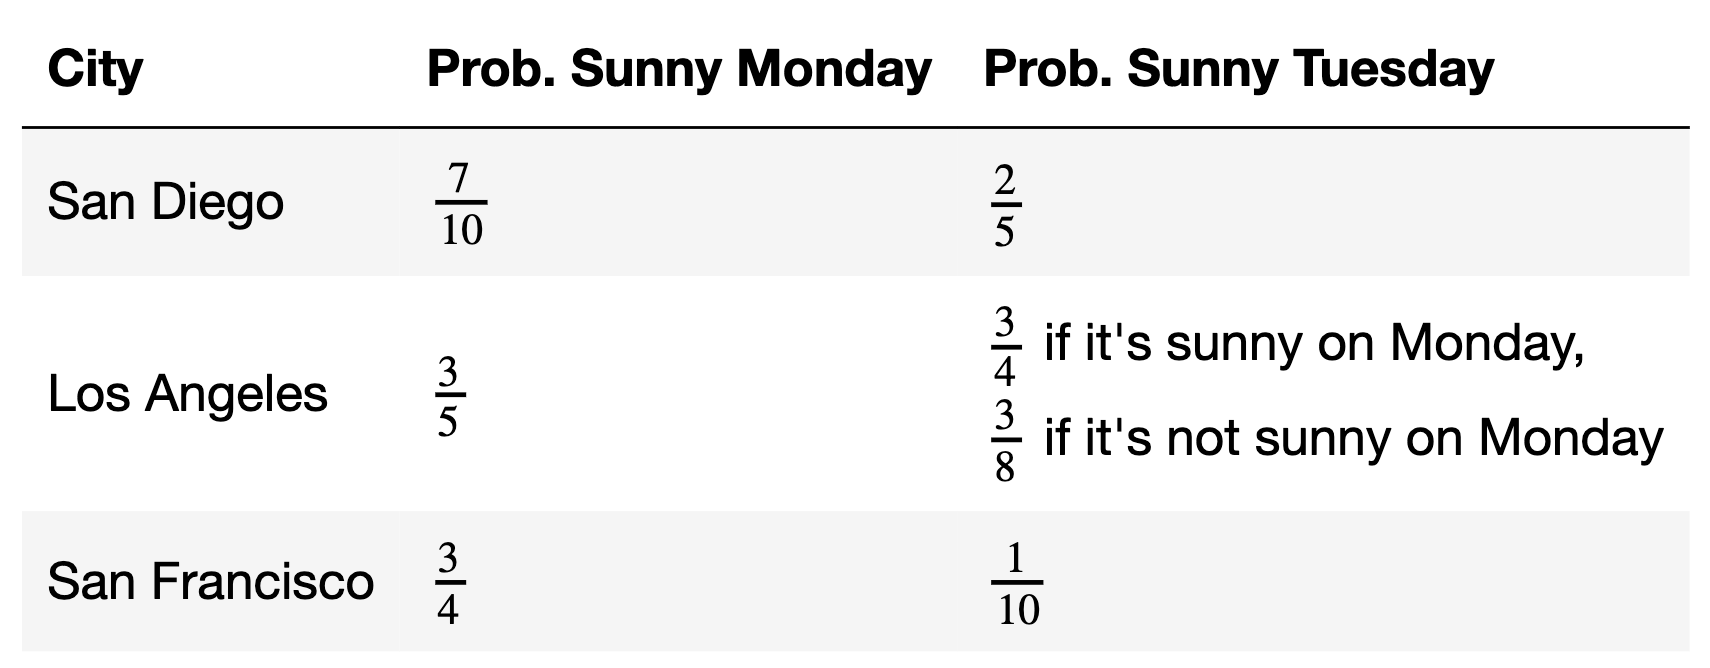
\includegraphics[width=0.7\textwidth]{final_images/probs-table.png}
\end{center}

\begin{subprobset}

\begin{subprob}(2.5 pts) What is the probability that it is not sunny in San Diego on Monday and not sunny in San Diego on Tuesday? Give your answer as a \textbf{positive integer percentage} between 0\% and 100\%.

\inlineresponsebox[2in]{}{}

\end{subprob}

\begin{subprob}(2.5 pts) What is the probability that it is sunny in at least one of the three cities on Monday?

\bubble{$3\%$}
\bubble{$31.5\%$}
\bubble{$40\%$}
\bubble{$68.5\%$}
\bubble{$75\%$}
\bubble{$97\%$}

\end{subprob}

\begin{subprob}(3 pts) What is the probability that it is sunny in Los Angeles on Tuesday?

\bubble{$15\%$}
\bubble{$22.5\%$}
\bubble{$40\%$}
\bubble{$45\%$}
\bubble{$60\%$}
\bubble{$88.8\%$}

\end{subprob}

% \begin{subprob}

% Suppose $q$ is your answer from the previous subpart. In terms of $q$, what is the probability that it is sunny on exactly one of Monday or Tuesday in LA?

% \bubble{$\frac{9q}{20}$} \bubble{$\frac{9}{20q}$} \bubble{$\frac{q}{2}$} \bubble{$\frac{1}{2q}$} \bubble{$\frac{3q}{4}$} \bubble{$q$} \bubble{$2q$}

% \end{subprob}

\newpage

\begin{subprob}(4 pts) Fill in the blanks so that \texttt{exactly\_two} evaluates to the probability that exactly two of San Diego, Los Angeles, and San Francisco are sunny on Monday.

\textit{Hint: If \texttt{arr} is an array, then \texttt{np.prod(arr)} is the product of the elements in \texttt{arr}.}

\begin{verbatim}
monday = np.array([7 / 10, 3 / 5, 3 / 4]) # Taken from the table.
exactly_two = __(a)__
for i in np.arange(3):
    exactly_two = exactly_two + np.prod(monday) * __(b)__
\end{verbatim}

What goes in blank (a)?

\begin{responsebox}{0.5in}
    
\end{responsebox}

What goes in blank (b)?

\bubble{\texttt{monday[i]}}

\bubble{\texttt{1 - monday[i]}}

\bubble{\texttt{1 / monday[i]}}

\bubble{\texttt{monday[i] / (1 - monday[i])}}

\bubble{\texttt{(1 - monday[i]) / monday[i]}}

\bubble{\texttt{1 / (1 - monday[i])}}
    
\end{subprob}

\end{subprobset}

\end{prob}

\newpage

\begin{prob}[(6 pts)]

Costin, a San Francisco native, will be back in San Francisco over the summer, and is curious as to whether it is true that about $\frac{3}{4}$ of days in San Francisco are sunny.

Fast forward to the end of September: Costin counted that of the 30 days in September, 27 were sunny in San Francisco. To test his theory, Costin came up with two pairs of hypotheses.

Pair 1:

\begin{itemize}
    \item \textbf{Null Hypothesis}: The probability that it is sunny on any given day in September in San Francisco is $\frac{3}{4}$, independent of all other days.
    \item \textbf{Alternative Hypothesis}: The probability that it is sunny on any given day in September in San Francisco is \textbf{not} $\frac{3}{4}$.
\end{itemize}

Pair 2:

\begin{itemize}
    \item \textbf{Null Hypothesis}: The probability that it is sunny on any given day in September in San Francisco is $\frac{3}{4}$, independent of all other days.
    \item \textbf{Alternative Hypothesis}: The probability that it is sunny on any given day in September in San Francisco is \textbf{greater than} $\frac{3}{4}$.
\end{itemize}

For each test statistic below, choose whether the test statistic could be used to test Pair 1, Pair 2, both, or neither. Assume that all days are either sunny or cloudy, and that we cannot perform two-tailed hypothesis tests. (If you don't know what those are, you don't need to!)

\begin{subprobset}

\begin{subprob}(1.5 pts) The difference between the number of sunny days and number of cloudy days

\bubble{Pair 1}
\bubble{Pair 2}
\bubble{Both}
\bubble{Neither}

\end{subprob}

\begin{subprob}(1.5 pts) The absolute difference between the number of sunny days and number of cloudy days

\bubble{Pair 1}
\bubble{Pair 2}
\bubble{Both}
\bubble{Neither}

\end{subprob}

\begin{subprob}(1.5 pts) The difference between the proportion of sunny days and $\frac{1}{4}$

\bubble{Pair 1}
\bubble{Pair 2}
\bubble{Both}
\bubble{Neither}

\end{subprob}

\begin{subprob}(1.5 pts) The absolute difference between the proportion of cloudy days and $\frac{1}{4}$

\bubble{Pair 1}
\bubble{Pair 2}
\bubble{Both}
\bubble{Neither}

\end{subprob}
    
\end{subprobset}

\end{prob}

\newpage

\begin{prob}[(11 pts)]

Raine is helping settle a debate between two friends on the ``superior" season --- winter or summer. In doing so, they try to understand the relationship between the number of sunshine hours per month in January and the number of sunshine hours per month in July across all cities in California in \texttt{sun}.

Raine finds the regression line that predicts the number of sunshine hours in July ($y$) for a city given its number of sunshine hours in January ($x$). In doing so, they find that the correlation between the two variables is $\frac{2}{5}$.

\begin{subprobset}

\begin{subprob}(1.5 pts) Which of these could be a scatter plot of number of sunshine hours in July vs. number of sunshine hours in January?

\begin{center}
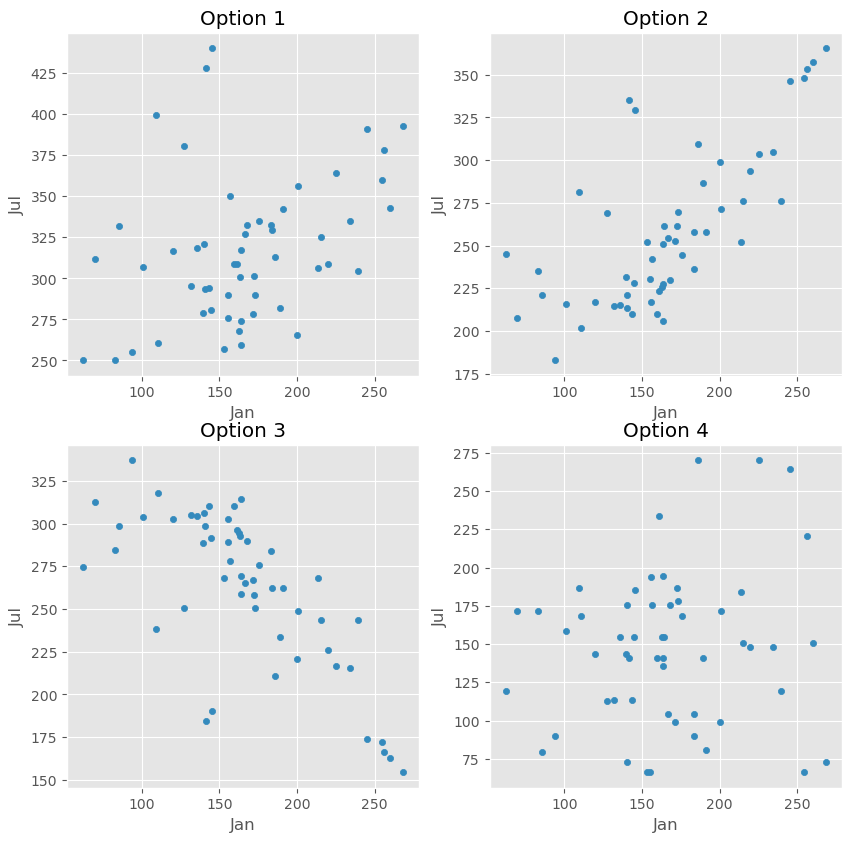
\includegraphics[width=0.7\textwidth]{final_images/r-values.png}
\end{center}

\bubble{Option 1}
\bubble{Option 2}
\bubble{Option 3}
\bubble{Option 4}
    
\end{subprob}

\newpage

\begin{subprob}(3 pts) Suppose the standard deviation of the number of sunshine hours in January for cities in California is equal to the standard deviation of the number of sunshine hours in July for cities in California.

Raine's hometown of Santa Clarita saw 40 more sunshine hours in January than the average California city did. How many \textbf{more sunshine hours than average} does the regression line predict that Santa Clarita will have in July? Give your answer as a positive integer. \textit{(Hint: You'll need to use the fact that the correlation between the two variables is $\frac{2}{5}$.)}

\inlineresponsebox[2in]{}{}
    
\end{subprob}

\end{subprobset}

As we know, San Diego was particularly cloudy this May. More generally, Anthony, another California native, feels that California is getting cloudier and cloudier overall.

To imagine what the dataset may look like in a few years, Anthony subtracts 5 from the number of sunshine hours in both January and July for all California cities in the dataset --- i.e., he subtracts 5 from each $x$ value and 5 from each $y$ value in the dataset. He then creates a regression line to use the new $x$s to predict the new $y$s.

\begin{subprobset}

\begin{subprob}(2 pts) What is the slope of Anthony's new regression line?

\inlineresponsebox[2in]{}{}

\end{subprob}

\begin{subprob}(3 pts) Suppose the intercept of Raine's original regression line --- that is, before Anthony subtracted 5 from each $x$ and each $y$ --- was 10. What is the intercept of Anthony's new regression line?

\bubble{-7}
\bubble{-5}
\bubble{-3}
\bubble{0}
\bubble{3}
\bubble{5}
\bubble{7}

\end{subprob}

\end{subprobset}

Jasmine is trying to get as far away from Anthony as possible and has a trip to Chicago planned after finals. Chicago is known for being very warm and sunny in the summer but cold, rainy, and snowy in the winter. She decides to build a regression line that uses month of the year (where 1 is January, 2 is February, 12 is December, etc.) to predict the number of sunshine hours in Chicago.

\begin{subprobset}

\begin{subprob}(1.5 pts) What would you expect to see in a residual plot of Jasmine's regression line?

\bubble{A patternless cloud of points}

\bubble{A distinctive pattern in the residual plot}

\bubble{Heteroscedasticity (residuals that are not evenly vertically spread)}
    
\end{subprob}
    
\end{subprobset}

\end{prob}